\chapter{Risultati Sperimentali}
La sintesi del componente viene eseguita correttamente e tutti i test vengono superati. Segue un piccolo approfondimento dei report e dei test bench.
\section{Report Utilization, Report Timing}
Com'è possibile osservare in \autoref{fig:Report} entrambi i report mostrano che il componente è stato implementato correttamente, non vengono inferiti latch e l'utilizzo del clock è ben al di sotto dei constraints.

\begin{figure}[!htb]
    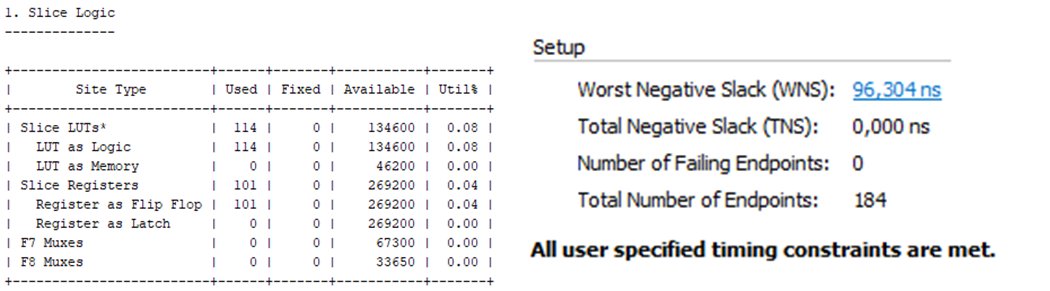
\includegraphics[keepaspectratio=true,scale=0.4]{images/Capitolo3/report.png}
    \caption{Il risultato dei report di Vivado}
    \label{fig:Report}
\end{figure}

In particolare il componente è composto da 101 Flip Flop, 0 latch e vengono utilizzati soli 4 nanosecondi a ogni ciclo di clock per completare le operazioni sui 100 disponibili.

\section{Test Benches}
Per verificare l’effettivo funzionamento del componente, esso è stato testato con numerosi test bench e con qualche test mirato sui casi critici nonostante la struttura del progetto non presenta molti corner case che non sono già richiesti all'interno della specifica. Qui di seguito si fornisce una breve descrizione dei casi più importanti.
\subsubsection{0 Byte da leggere}
Il caso in cui i Byte da leggere sono 0 il componente si comporta correttamente, esso non fa partire la convoluzione e termina il processo.
\begin{figure}[!htb]
    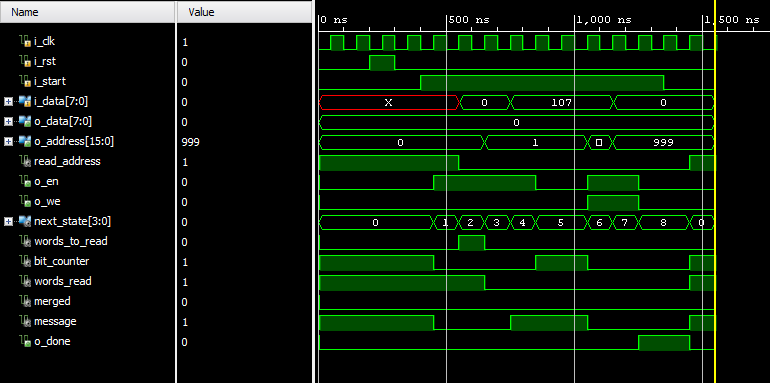
\includegraphics[keepaspectratio=true,scale=0.7]{images/Capitolo3/min.PNG}
    \caption{Lo schema dei segnali nel caso in cui non ci siano parole da leggere}
    \label{fig:signal1}
\end{figure}
\subsubsection{255 Byte da leggere}
Il caso in cui i Byte da leggere sono il massimo richiesto il componente non presenta criticità ed esegue la convoluzione correttamente.
\begin{figure}[!htb]
    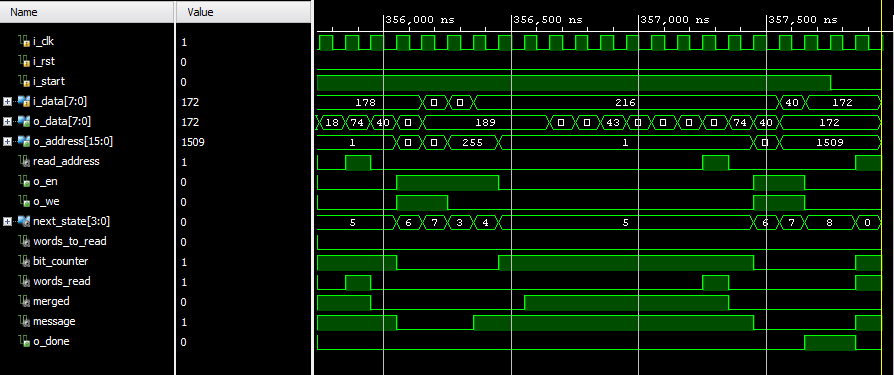
\includegraphics[keepaspectratio=true,scale=0.65]{images/Capitolo3/max.PNG}
    \caption{Lo schema dei segnali nel caso in cui la sequenza di parole da leggere è 255}
    \label{fig:signal2}
\end{figure}
\subsubsection{Due o più codifiche senza reset intermedio}
Nel caso in cui si vogliono eseguire più convoluzioni consecutive è necessario tenere conto che il componente deve essere pronto senza ricevere in ingresso un segnale di reset. Il componente realizzato rispetta la specifica e non ha problemi a gestire convoluzioni multiple.
\begin{figure}[!htb]
    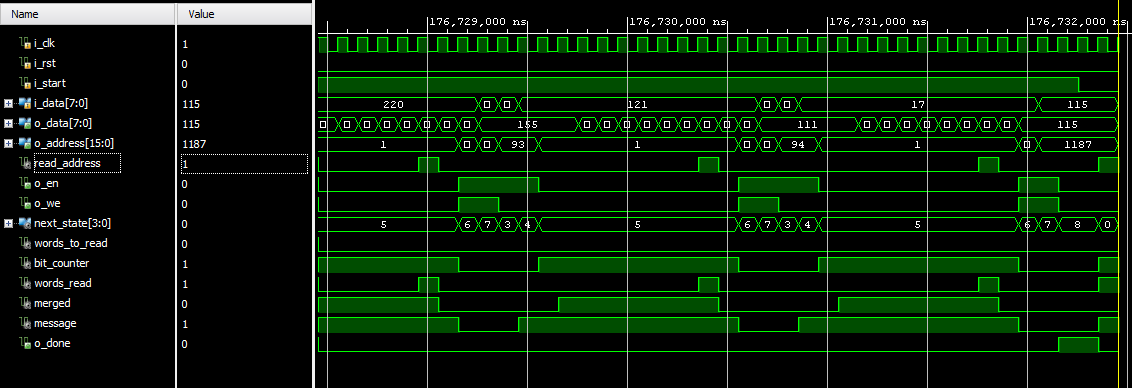
\includegraphics[keepaspectratio=true,scale=0.5]{images/Capitolo3/noreset.PNG}
    \caption{Lo schema dei segnali in un caso di codifiche multiple}
    \label{fig:signal3}
\end{figure}

\section{Conclusioni e Scelte Progettuali}
Si è giunti quindi alla conclusione che il componente realizzato rispetta pienamente le specifiche ed è stato accuratamente testato.

Si è deciso di utilizzare un registro per memorizzare l’indirizzo in cui leggere, e di non memorizzare quello in cui scrivere poiché viene ricavato in fase di esecuzione. Questo permette di avere un architettura più chiara e di risparmiare sull’utilizzo di qualche registro.